\chapter{Design Motivations}
\label{Motivations}

\par Being a mathematician and not a programmer, I wanted as general of a solution as possible to creating an extensible and multi-use simulation model.  After all--if one can prove that the generalized solution works, then any special case should, too.  So I set out redefining the problem of traffic simulation from a data structures and storage problem to one of pure graph theory and combinatorics. \\

\par  However, it wasn't very long before I was forced to face the fact that computers do not quite work like that, and computers require a bit more work to conform to the natural mathematics of graph theory.  While computers force discreteness, I aimed to design a simulation system which could mimic real-world continuity as closely as possible.  With that as the utmost goal, the system was designed as follows: \\

\section{Network Structure}
\par At least my computer and I could agree on one thing from the start:  traffic simulation is a graph problem.  Intuitively, nodes are connection points for several edges, like road intersections, cellular towers, etc.  By utilizing graph data structures, one can also take advantage of the numerous existing path-finding algorithms and easily keep track of connected pair of nodes (and their directionality). \\

\par Further continuing with intuitive design decision, it followed that the network needed to be directional, and that multiple parallel edges between a pair of nodes should be allowed.  Directionality's reason is easy to sport:  car lanes force traffic in a particular direction, and packets of information cannot necessarily be transmitted in both directions (especially if there are intermediary steps, like encryption, that are not reversible). \\  

\begin{figure}[H]
    \centering
	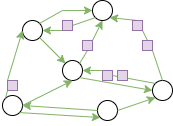
\includegraphics[width=0.5\textwidth]{tex files/Figures/generic_network.png}
	\caption[Random directional network]{Random directional network with objects on it}
	\label{fig:generic_network}
\end{figure}

\par Redundancy is a bit trickier, but ensures that this traffic simulator has the flexibility to model microscopic and macroscopic traffic trends \cite{LWB18}.  Allowing for multiple parallel edges is a good way to increase (or restrict) edge capacity, and serves as another parameter the user can tune to mimic real-world constraints.  Using normal commuting traffic as an example, a user can test whether or not adding another lane to a freeway (or adding lane accessible to cars only of a certain type) would ease congestion as they are able to view metrics and positionality per timestamp of the entire system (macroscopic), the set of edges between two nodes or each individual node (mesoscopic), and the individual cars on those roads themselves (microscopic) \cite{LWB18}. \\


\par Though some traffic simulations in existence use adjacency matrices to define neighbouring nodes \cite{GPK02}, this is not a scalable, nor desirable, solution.  While adjacency matrices are intuitive for humans to read and understand, since most networks are fairly sparse they end up storing a lot of NULL values.  While little heed is paid to memory conservation in the rest of this simulation's design process, the idea of holding space for nonexistent edges did not seem like a very good idea.  Instead, it makes sense to think more about the interactions of node-edge sets.  Adjacency matrices acknowledge that an edge is defined by its originating and terminal nodes, but fails to demonstrate how a node is only interesting because of the set of inbound and outbound edges it connects.  To capture both of these ideas, I used dictionary mappings to identify and link nodes to edges and edges to nodes, allowing either or both interactions to be utilized, depending whichever one was more intuitive for the particular action being done at any point in the simulation process.\\



\section{"You Are Here"}

\par A traffic simulation is not very insightful without considering the things which themselves cause traffic--Who, or what, keeps track of where the "cars" are?  Though innocuous, the question leads to some philosophical fancies that need to be addressed before determining who (or what) is in charge of your position. \\

\par If you're driving home at midnight, you might choose to take a faster route or a more scenic route, you might pull over to look at the citylights or take a pause because you're feeling sleepy, or you might drive a bit over the speed limit up because there's not likely to be any cops on the road at this hour of night.  It feels like you own the road and you have full control over where you are right here right now.  \\

\par But what if you (are trying to) drive home 5 o'clock Friday in the thick of traffic?  Yes, you \textit{chose} to take a particular route home, but now you're stuck in bumper-to-bumper traffic and can't move forward til the car in front of you decides to (or can at all).  While you may be in control of your car, you don't have full control over your ability to move, and thus over your position.  This leads to the inevitable conclusion that a simulation will be most accurate if the network controls the cars rather than letting the cars control themselves, meaning that current position must be stored on the objects over which the cars are moving:  the edges.

\section{...But where, exactly, is "Here"?}

\par Since edges store car locations and move them along a particular distance each unit of time, it's tempting to think of positions in terms of capacity.  If an edge is 10 units long and cars travel 2 units per time, there are 5 positions a car can be, so a car's position can be stored as its index in the capacity queue.  This makes movements easy to simulate and requires a minimal, fixed storage space no matter the amount of cars on the network.  So this is that design choice, right? \\

\par ...well, not quite.  Sure, the example above is easy to quantify, but breaks down when situations arise that obstruct predictable movement, ranging from traffic jams to even just switching to an edge with a different speed limit.  If a car is unable to move its full potential, it's then unable to move into the next discrete state.  So where does it go? And where do any cars after it go? \\

\par The problem with defining position by the distance a car can go at it's maximum speed is that there's a lot of unaccounted distance.  If a car is going 10 m/min, then the position would be defined as 10 meters later (if the unit time distance of the simulation were in minutes)--in a road stretch of 60 meters, there would be 6 possible positions.  \\

\begin{figure}[H]
    \centering
	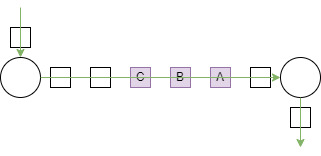
\includegraphics[width=0.75\linewidth]{tex files/Figures/BasicDiscrete_Before.png}
	\caption[Discrete positions: example]{Example discrete system with 6 slots, 3 of which currently occupied}
	\label{fig:BasicDiscrete_before}
\end{figure}


\par Now let's say that the car (car A) has reached the end of the road segment and is trying to turn onto a crossroad, but the crossroad is completely full.  Car A must stop at the end of the road segment and wait for an opening.  The car behind (car B), meanwhile, is still driving 10 m/min but must stop before crashing into the halted car in front, but any cars behind it are still capable of moving fully into the next position in the queue.  Where is Car B?  It cannot be in the final position (as Car A is still occupying it), and the penultimate position is now taken up by Car C which was one position behind Car B.\\

\begin{figure}[H]
    \centering
	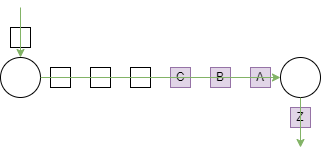
\includegraphics[width=0.75\linewidth]{tex files/Figures/BasicDiscrete.png}
	\caption[Discrete positions: blockade]{No obstructions yet:  all cars have proceeded one slot forward}
	\label{fig:BasicDiscrete}
\end{figure}


\par Faced with this situation in a discrete system, we must compromise on simulation accuracy:  either you allow cars to pile up on positions (defeating the purpose of a queue \textit{and} unrealistically depicting car location), or you prevent cars from moving at all (artificially causing traffic on the current edge when there is, in fact, room to move.  This cascades onto other connected edges and may stall the whole simulation).  While option one doesn't seem too terrible, it runs the risk of allowing cars to "jump" over halted cars; if car C's destination is the location car A is stuck, then when car C piles onto the position two timestamps later, it registers as completing its journey despite that being impossible in a real-world scenario.  \\

\begin{figure}[H]
    \centering
	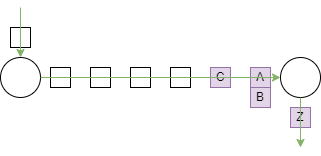
\includegraphics[width=0.75\linewidth]{tex files/Figures/BasicDiscrete_Overlap.png}
	\caption[Discrete positions: multiple cars at one location]{Car A is stuck, car B and C advance, causing car B to share a spot with car A}
	\label{fig:BasicDiscrete_overlap}
	
	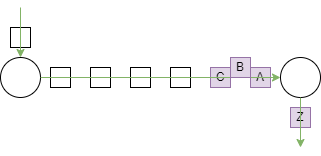
\includegraphics[width=0.75\linewidth]{tex files/Figures/BasicDiscrete_between.png}
	\caption[Discrete positions: non-fixed locations]{Car A is stuck, car B advances to an in-between stage, Car C advances one slot forward}
	\label{fig:BasicDiscrete_between}
\end{figure}

\par It is clear that some other solution is needed if a realistic simulation is to be created.  And that solution is simple:  switch to floating point positions.  By mapping cars to their exact position from 0 to maximum edge length, the user can be explicit about how long each car is and how close the cars are allowed to be to each other, all the while ensuring accuracy in car behavior by preventing skipping.


\section{Paths, Origins, and Destinations}

\par "How do I get from Point A to Point B?" and what even constitutes a "point"?  Path-finding algorithms typically find the fastest/shortest/"best" route between any 2 given nodes, which would imply that nodes are the points. This intuitively makes sense and works great for simulation paths with bounded, real-world constraints.  Take (a very simplified example of) email communication:  emails will always start at one machine (node), travel to a server (node), and perhaps be passed onto another server for the receiver to view (node); there might be more or less steps between each landmark, but the only way the message can get lost as at one of the endpoints.  \\

\par However, cars do not spawn in the middle of a four-way intersection, nor does it make sense to create a network model where every possible parallel parking spot is a separate node in a network.  For one, someone could do a terrible parking job and take up two spots, therefore creating some new start or end node somewhere between the existing spots.  But the more pressing issue with breaking a road into n continuous, sequential, connected segments is the same sort of unwanted inefficiency as the adjacency matrices proposed earlier:  there's a lot space and computation wasted on pairs that generally provide no function to the simulation. \\

\par This led me to turn the usual graph structure on its head, and instead allow cars to enter and leave the network from the edges themselves.  To make this work for traditional node-to-node paths, the car placement mechanism has been written in such a way that if no specific edge location has been specified for a start and end point, a path is selected based on those nodes and the "car" is placed at position 0 along the first edge (and finishes its journey at the maximum length of the final edge, or effectively at the terminal node). \\

\par Since start and end locations have been set to edges, path finding calculations also are done on an edge to edge basis.  As edges only know their bounding nodes (and nodes their adjacent edges), calculations are done on the network level, allowing chaining between edge dictionaries of nodes and node dictionaries of edges to build potential paths.


\section{Order}

\par A methodical process is needed to execute all the actions that can take place on each tick of the simulator (tick being the function that executes said changes for each incremental timestamp in the simulation runtime). \\

\par The network object is build of nodes and edges, so it makes sense to break down the action queue to these levels as well.  However, you can't just arbitrarily run all nodes and edges as there is an inherent order and hierarchy to them.  As edges are defined by their start and end nodes, it makes sense to have edge tick processes as a dependent of node tick processes.  Furthermore, because nodes are capable of having multiple inbound and outbound edges, it is essential to process a particular node's edge ticks together to ensure as smooth and realistic of a movement between edges as possible. \\

\par To ensure that each component of a network is only processed once, on each tick, the network tick function iterates through all nodes listed in the network's node dictionary.  Each node, in turn, processes each outbound edge in its adjacent outbound edges dictionary.  The network tick and its subsequent node and edge ticks will be performed as many times as necessary until the cars run out of energy \textit{or} no more advances can be made with the current remaining energy potentials, and report out the number of loops needed to do so and the total percent of potential energy used.  These values can be used as a proxy for network congestion, though more as a benchmark between ticks or simulations than as an absolute value of ability. \\

\par To ensure that no node nor edge is favored (ei: always has their candidate cars move before any other node or edge's), the order in which these items are iterated is shuffled with each pass.  While this helps immensely with simulation accuracy, the random nature is what prevents the output numbers from being a reliable and accurate metric of network (in)action. 


\section{Movement}

\par A simulation is practically useless unless it models the movement of objects predictably and (semi-)realistically; the problem of how to model node-crossing caused me quite some consternation. \\

\par  For an intersection consisting of one inbound edge and one outbound edge, the logic is simple:  when a car reaches the end of one edge, check the following edge and place it there if there is room.  Even in the simple scenario, there are certain complexities that arise when translating that from math theory to computer code, and compound when adding more degrees of freedom by adding more inbound and outbound edges: 

\begin{itemize}
    \item What counts as "room"?
    \item How far does a car go on to the following edge?
    \item What if the two edges have different speeds?
    \item What if cars from two (or more!) different inbound edges want to move onto the same new edge?
    \item Are cars allowed to change their path?
\end{itemize}

\noindent And this list doesn't even consider what happens what other optional attributes like stoplights are added into the mix!\\

\par "Room" is the easiest to answer and was already hinted at a few sections ago:  a car will move as far as it possibly can, given the internal and external constraints on its movement.  This holds for movement within a given edge and across edges (node-crossing).  \\

\par In describing why a discrete system didn't work, I used the word "potential" to describe a car's possible range of movement; this was not on accident.  Even on a floating-point system, the maximum distance a car is allowed to go in one unit of time (tick) is an essential calculation for determining all aspects of a car's movement.  I describe this value as "maximum\_tick\_potential".  Leaning into the field of physics:
\begin{itemize}
    \item "Work" is defined as the amount of energy expended to move a certain distance in a certain period of time.
    \item An object at rest has some arbitrary value of potential energy.  
    \item The law of conservation of energy states that energy can neither be created nor destroyed.
\end{itemize}

\noindent It follows that the total energy of the universe remains constant, so any energy expended on moving an object is subtracted from the object's potential energy to ensure the balance remains.  By defining a car's "potential" for movement during one tick, we can define its actual moment as a proportion of that, allowing multiple actions to be done in one tick (as long as there is energy potential to spend).  Furthermore, we can calculate the total unexpended energy at the end of the tick of the entire network \textit{or} for a particular edge and use this as a metric for how backed-up or congested the network is. \\

\subsection{Car Movement Using Tick Potential}
% TODO:  illustrate with drawings
\par The following steps describe how a car can possibly move within one tick.
\begin{enumerate}
    \item Each car starts with it's maximum potential energy at the start of a tick (default = 1).  This is the currently available potential energy.
    \item Any car that takes an action on the list below is done moving for the current tick and will be moved from the current\_cars queue to a processed\_cars queue.
    \item If a car has been added to the simulation and is waiting to enter the network, check if its start position is open, and add it to the edge at the location if possible (or keep it in the waiting queue if not).  Placement on the edge uses up the full energy potential to prevent cars that enter late in the network tick loop from moving more than is realistic.
    \item Evaluate how far a car can possibly move along its current edge:  The maximum possible distance is the edge's speed limit times the currently available potential energy, but the actual possible travel distance is that to any obstacle in front of it.  If there is a car in front, the car can only move to behind it; if the edge ends, the car can only go to the end at the current speed; if the car reaches its path end position, it leaves the network entirely; otherwise, the car can go its full potential.  
    \item Calculate the work done to get to that position:  divide distance travelled by maximum potential distance (speed limit).
    \item Subtract work done from the remaining available energy (or maximum potential energy).  If there is still energy left and a car has reached the end of the current edge, proceed.  Otherwise, wait til the next tick.
    \item Evaluate if the car can proceed on to the next edge:  nodes might have a (time) penalty for crossing (such as time to physically cross an intersection); if the car does not have enough energy left after "paying" this penalty, then the car cannot proceed further and must wait til the next tick.
    \item Select the next edge in the path:  for some cars, this is simply the next edge in the path list; other cars (depending on car type) may require a calculation to choose a new path first.
    \item Repeat steps 3 through 8 as long as there is energy remaining \textit{or} until the car is forced to wait.
    % \item Once no more movement is possible for the current tick, concatenate set processed\_cars lists as the new current\_cars queue for next tick.
\end{enumerate}

\subsection{Multiple Inbound Edges}
% TODO:  illustrate with drawings
\par The issue of multiple cars across several edges eligible to change onto the same new edge is solved, in part, by the random shuffling of each node tick and edge tick order.  Some randomness will persist as the order edges are processed may affect whether other cars are even eligible to enter after it, but I would argue that the randomness accurately portrays real-world indecisiveness (at least for car traffic networks) and thus is not something to fear, but rather embrace.  However, if this is deemed undesirable by the user, they can mitigate the effects by choosing a small enough tick time that differences are negligible.  Tick time can be adjusted by adjusting the scalar values for the maximum speed parameter of the edges.


\section{Attributes}

\par Since the simulation software should allow for full flexibility in what types of network systems it models, it was important to make sure the simulation requires as few mandatory fields as possible to produce a reasonable simulation, but allow for additional parameters inherent to a particular system.  \\

\par Following basic graph theory, the essential attributes for the network (nodes and edges) itself is only what is strictly required to make a graph:  a unique identifier per object, and for edges a value to link each end to it respective node. However, a slew of additional attributes (like delay for nodes or maximum capacity for edges) can be specified to make the traffic model more complex, adapting parameters and interactions to more closely model a specific real-world system of choice.



\section{Snapshot}

\par Though the random factor prevents a truly reproducible simulation, I have designed the simulation snapshots to be made in such a format that they can also serve as simulation input for later simulation.  This provides continuity between all files associated with the simulation and makes it easier to recover the simulation and its output in case of machine failure/crashing. \\

\par Snapshots output a human-readable dump of the entire simulation state, including all details on cars, edges, and nodes.  It was important to me that the user be able to obtain these snapshots whenever they like, allowing the flexibility to save every single tick state (and maybe dump to a database for detailed analysis), or only final or important interim states if desired.